\chapter*{Knowledge Graph Visualization Tool}
During the process of working on the master's thesis, we were searching for a framework that could visually represent our implemented knowledge graph. Our aim was to clarify the connections and relationships between individual classes. In our search, we found several interesting frameworks that seemed suitable for our needs, which are also mentioned in the Related Work chapter. NOTE RELATED WORK HERE.

However, these solutions weren't entirely satisfactory for us because they lacked some tools that we deemed important. Therefore, we decided to develop our own tool, which should serve as a good visualization framework for our and similar use cases.

In this chapter, we present the framework we developed, from the initial idea to the implementation and the functionalities of our tool.

\section*{Main concept}

Wir entschieden uns für 3 Hauptkomponente, welche das neue Framework beinhalten sollte:
\begin{itemize}
    \item Klare Visualisierung: Um die Navigation durch den Wissensgraphen zu erleichtern, setzten wir uns als erstes Ziel, die Relationen und Klassen des Graphen so deutlich wie möglich hervorzuheben. Dies könnte zum Beispiel durch die Nutzung verschiedener Farben für verschiedene Klassen passieren oder durch das Highlighten einer Klasse und die dazugehörigen Klassen zu denen eine Relation besteht.
    \item Query Builder: Um die Relationen zwischen den Queries zu verdeutlichen, benötigen wir einen Query Builder, der gegeben einer Klasse, durch die Relation auf andere Klassen hinweisen kann, welche wiederrum durch eine weitere Relation auf weitere Klassen hinweisen kann, solange wie der Nutzer das möchte oder es keine weiteren Relationen gibt. Dies sollte geschehen ohne die Query Sprache SPARQL einsetzen zu müssen, wodurch es dem Nutzer um einiges erleichtert wird.
    \item Inference Query: Da unsere Arbeit auf Inferenzen beruht, möchten wir eine Inferenz Query implementieren, welche durch den Input einiger Klassen, auf inferierte Parameter hinweisen kann. Dieser Anwendungsfall ist ziemlich spezifisch für unseren UseCase, allerdings sollte dies auch auf andere Ontologien abbilden können. Der Output sollte ein Aktionsbaum sein, mit den inferierten Parametern und einen visualierten Graphen mit den dazugehörigen Klassen, welche für die Inferenz eine Rolle spielen.
\end{itemize}

\subsection*{Architekturbeschreibung, briefly}

Die Architecture besteht aus einem Full Stack Framework, welches im Backend das WebFramework Flask benutzt und fürs Frontend HTML und JavaScript. Für das Styling des HTMLs nutzen wir eine abgeänderte Version von Bootstrap. Außerdem werden im Backend die Bibliothek rdfLib genutzt um Daten aus der Wissensbasis zu verarbeiten. Die JavaScript Funktionen sind für die Visualisierung des Graphen da, welches mit der JS Bibliothek "Vis.js" geschieht.

Die folgenden Grafiken soll eine einfache Beschreibung der Architektur visuell darstellen, sowie die Ordnerstruktur anzeigen.
\begin{figure}[!ht]
    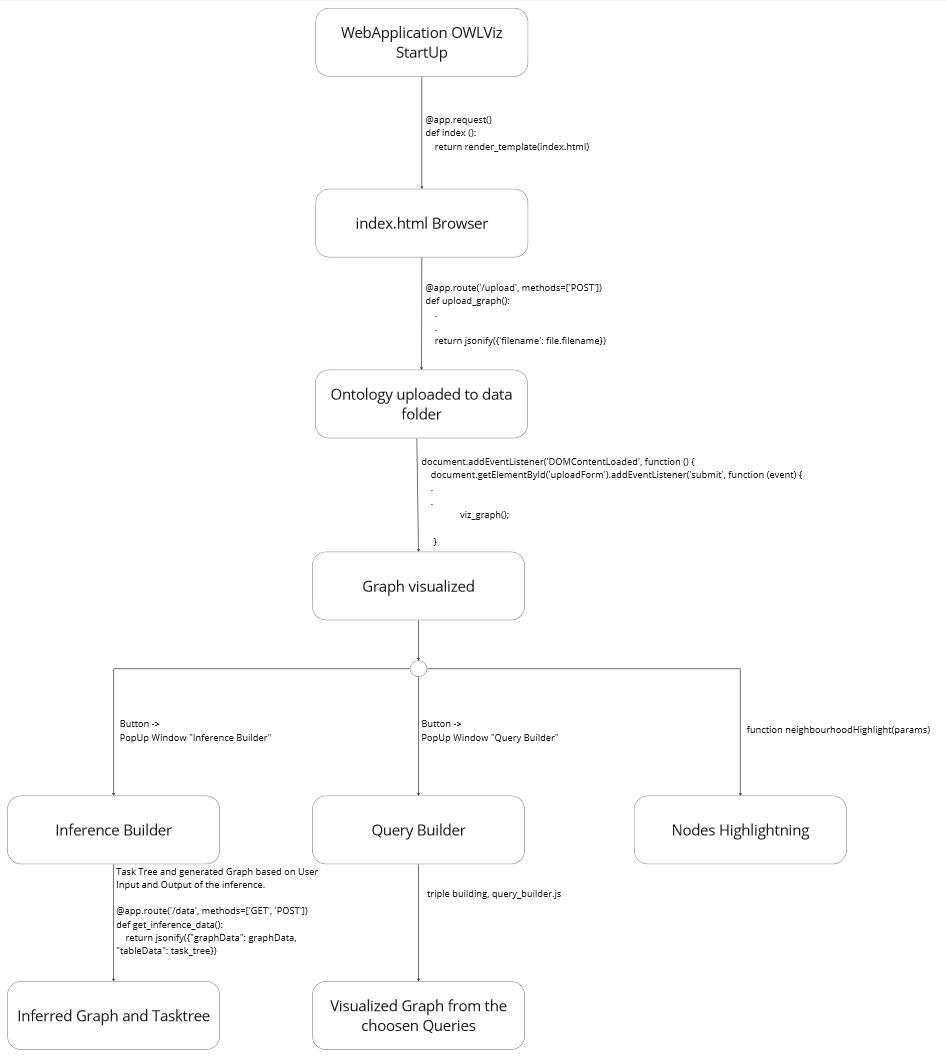
\includegraphics[scale=0.35]{Graphics/OWLViz_architecture.jpg}
    \end{figure}

\dirtree{%
.1 main.py.
.1 templates.
.2 index.html.
.1 data.
.1 static.
.2 graphviz.js.
.2 query\_builder.js.
.1 src.
.2 graph.
.3 graph.py.
.3 coloring.py.
.3 graph\_utility.py.
.2 inference\_builder.py.
.2 query\_builder.py.
}

Im Folgenden wollen wir auf die einzelnen Punkte der Architektur aus einer TopLevel Sicht näher betrachten.

\subsubsection*{WebApp StartUp} 

Um die Anwendung zu Starten muss das Python Skript \textit{main.py} ausgeführt werden.
Dies kann mit dem folgenden Command, soweit die benötigten Bibliotheken installiert wurden, ausgeführt werden.

\textit{\$: python main.py}

Damit wird die Flask Webanwendung gestartet und die Startseite \textit{index.html} aufgerufen.

\begin{figure}[!ht]
    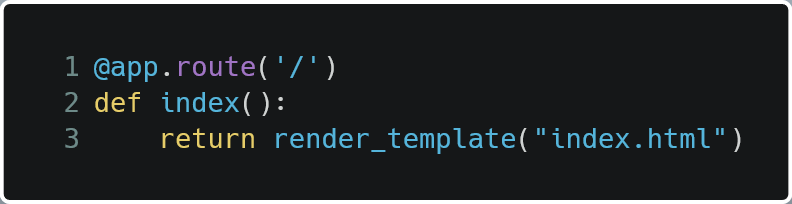
\includegraphics[scale=0.35]{Graphics/def_index.png}
    \end{figure}

    \begin{itemize}
        \item \textit{@app.route("/")} zeigt an, welche Funktion als erstes beim Starten des Frameworks ausgeführt wird.
        \item \textit{render\_template("index.html")} diese Funktion zeigt welche HTML-Seite dabei aufgerufen wird, in diesem Fall \textit{index.html}
    \end{itemize}

\subsubsection*{Upload Ontology}

Die WebApp startet erstmal mit einer (fast) leeren HTML-Seite, welches nur über einer Navigationsbar verfügt.
Dem Nutzer steht jetzt die MÖglichkeit zu, selbst eine Ontologie hochzuladen, um mit dieser weiter zu arbeiten.
Die Funktion \textit{upload\_graph()} speichert die Ontologie im \textit{data} Ordner.
\begin{figure}[!ht]
    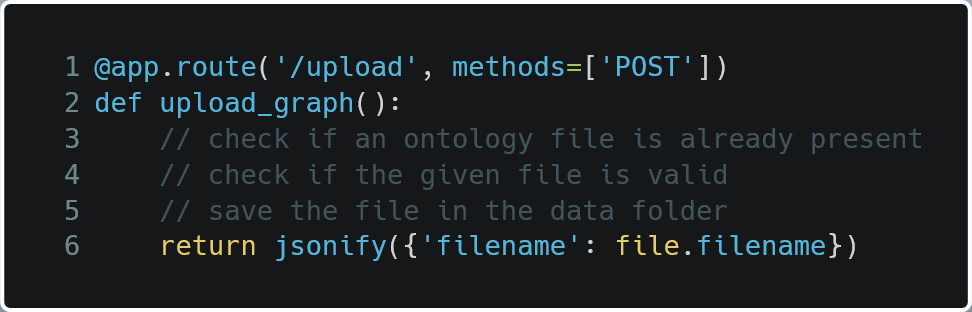
\includegraphics[scale=0.2]{Graphics/upload_graph.png}
    \end{figure}

\subsubsection*{Visualized Graph}

Wenn die Ontologie hochgeladen wurde, wird die JavaScript Funktion \textit{viz\_graph()} ausgeführt, welche letzendlich den Graphen visualiert.
Diese Funktion fetcht die benötigten Knoten- und Kantenmengen aus der BackEnd Funktion \textit{get\_graph\_data()}

\begin{figure}[!ht]
    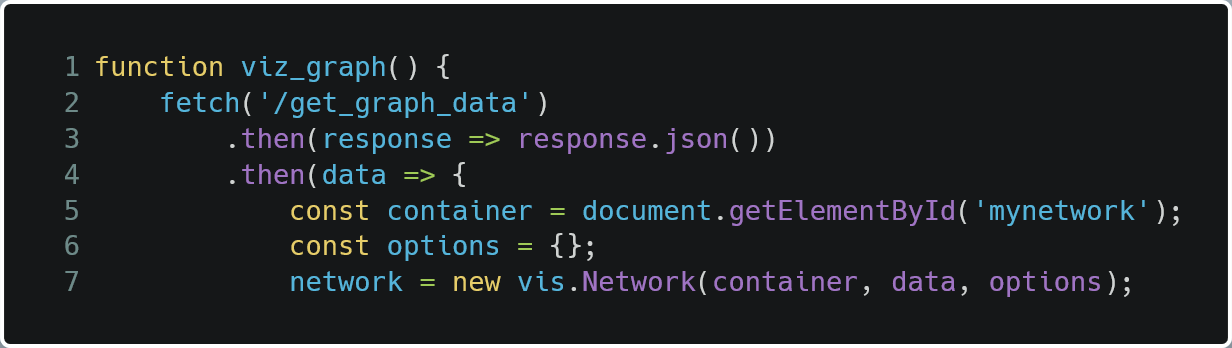
\includegraphics[scale=0.2]{Graphics/viz_graph_function().png}
\end{figure}

\begin{figure}[!ht]
    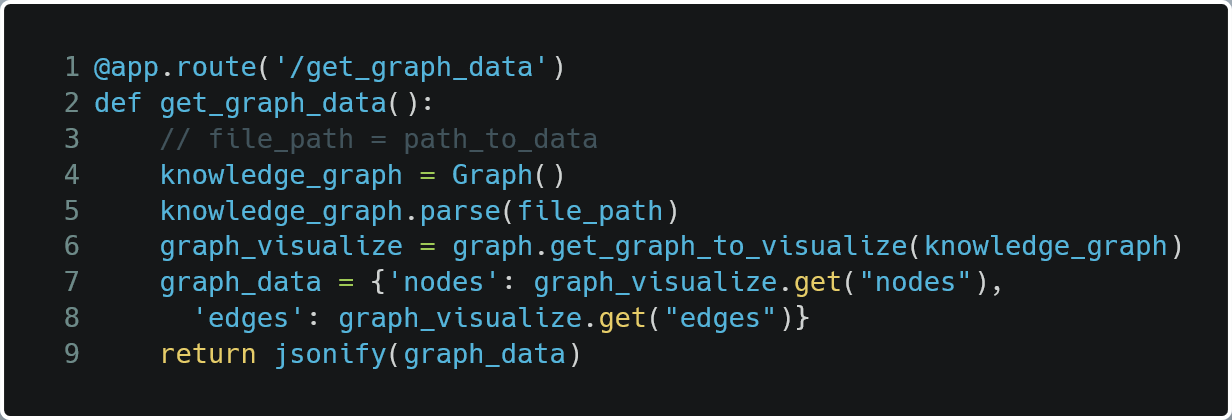
\includegraphics[scale=0.2]{Graphics/get_graph_data.png}
\end{figure}

Die Verarbeitung der Daten ist komplex und wird im Kapitel Implemetierung (HINWEIS KAPITEL Implemetierung) näher ausgeführt.
Außerdem haben wir einen Abschnitt geschrieben, welches eine einfache Einführung in unser Framework geben soll, dieser soll mit einem einfachen Beispiel die Funktionsweisen verdeutlichen (HINWEIS EinführendesBeispiel).

\subsubsection*{Nodes Highlightning}

Bei großen Graphen, kann es schwierig werden die Übersicht über die Knoten und dazugehörigen Relationen zu behalten. Deshalb implementieren wir eine Funktion, welches einen Knoten, sowie die benachbarten Knoten highlighted.
Dies soll dazu führen, dass man einfacher den Überblick über eine Klasse und die dazugehörigen Relationen erhält.
Die dazu benötigte Funktion ist eine JavaScript Funktion, welche als Parameter einen angeklickten Knoten nimmt, und darauf basiert die benachbarten Knoten berechnet. Anschließend werden alle Knoten
ausgegraut, und der ausgewählte Knoten und seine Nachbaren, bekommen die ursprüngliche Farbe zurück. Dadurch erscheinen die ausgewählten Knoten "gehighlighted".
\begin{figure}[!ht]
    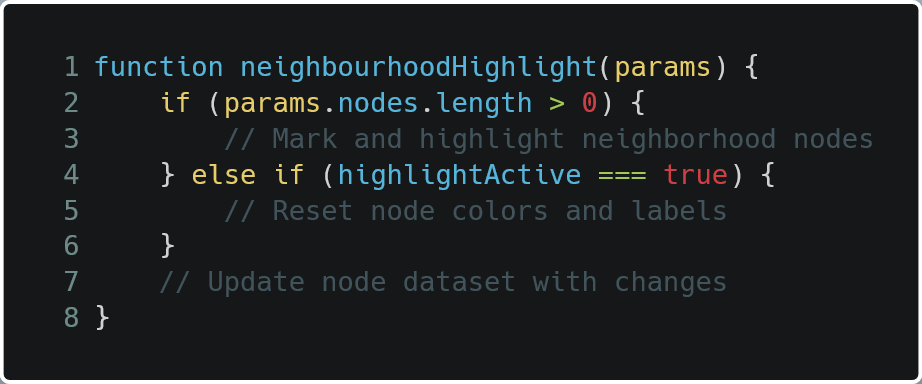
\includegraphics[scale=0.3]{Graphics/neighbourhood_highlighting.png}
\end{figure}

\subsubsection*{Query Builder - Naser}

\subsubsection*{Inference Builder}
Die letzte Möglichkeit für den Nutzer, Funktionen auf einem Graphen auszuführen ist der Inference Builder.
Vorab gesagt, der Inference Builder ist kein generischer Anwendungsfall und ist in dieser Version auf dem Mixing Graphen (HINWEIS HIER) abgestimmt.
Im Kapitel Implemetierung (HINWEIS HIER), wird die ImplemetIierung näher erklärt und aufgezeigt wie dies auch für andere Ontologien eventuell implementiert werden kann.
In unserem Fall inferieren wir eine Motion und dazugehörige Parameter basierend auf einer gegebenen Task und einer belieb langen Liste von Zutaten.
Der Inference Builder generiert dann einen Graphen, welche nur die dazugehörigen Knoten übersichtshalber anzeigt, sowie einen Tasktree der von einem Agenten befolgt werden kann.

Im ersten Weg werden der Task und die Zutaten an das Backend für die Inferenz gesendet, welches wiederrum dann die inferierten Motion und Parameter zurück an das FrontEnd schickt.

\begin{figure}[H]
    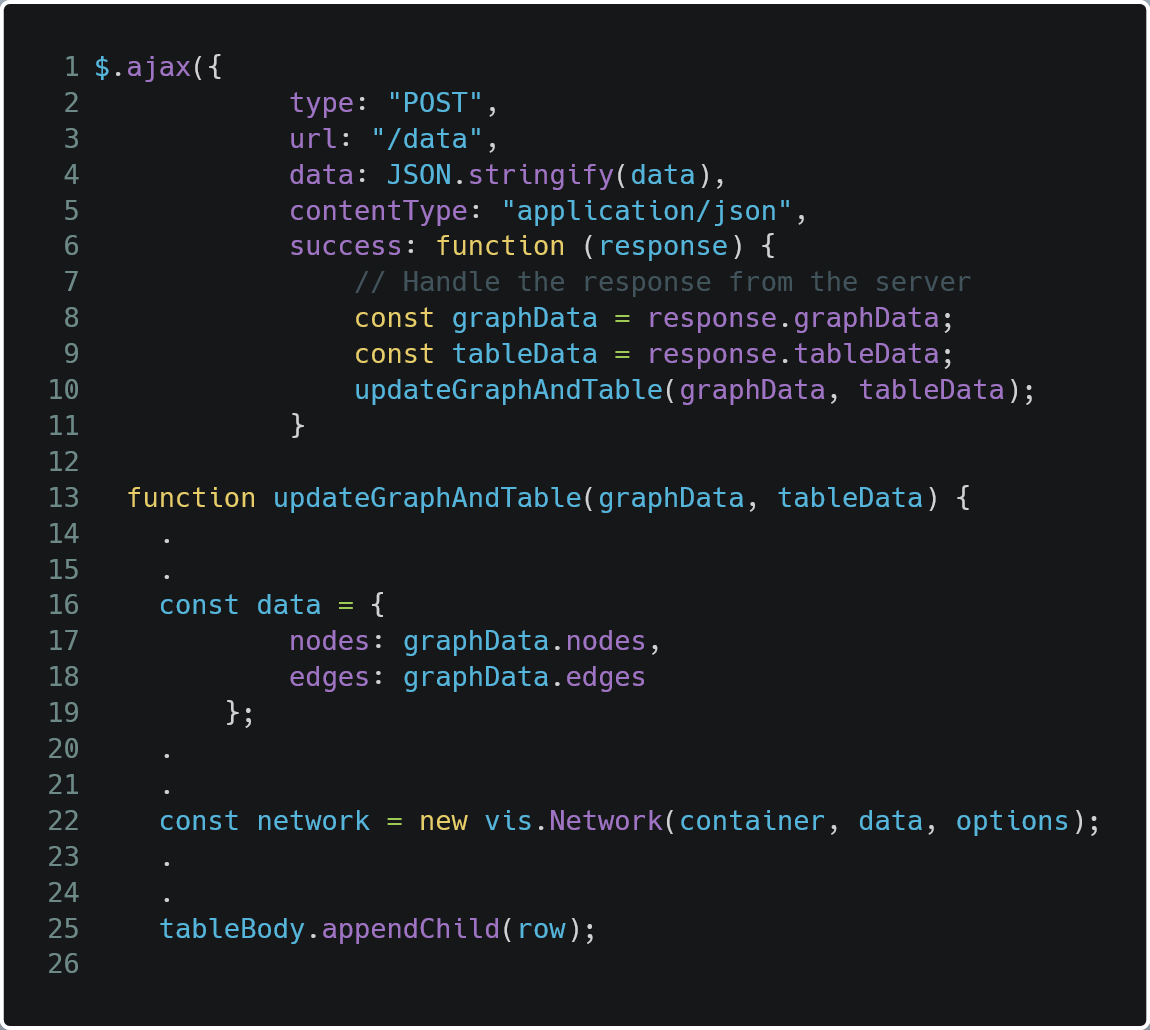
\includegraphics[scale=0.25]{Graphics/inference_builder_js.png}
\end{figure}

Die BackEnd Funktion verarbeitet die Inferenz mit den empfangenen Parametern, welche dann für die Visualisierung genutzt werden.

\begin{figure}[H]
    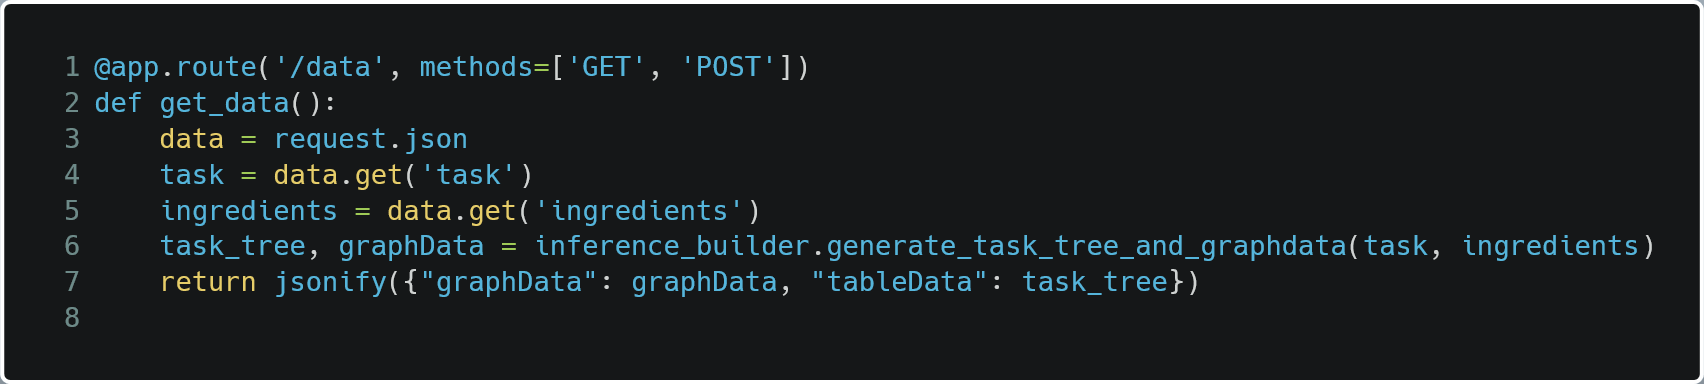
\includegraphics[scale=0.25]{Graphics/get_data.png}
\end{figure}
\subsection*{Einführendes Beispiel des Frameworks}
In diesem Abschnitt stellen wir ein einfaches Beispiel unseres Frameworks dar, von der Verarbeitung der Ontologie, bis zur Visualisierung in der Webanwendung.
Dies soll für den Leser den Einstieg in unser Framework erleichtern. 
Für diesen Zweck erstellen wir eine kleine und einfache Ontologie, um die Programmabläufe unkompliziert erklären zu können.
Außerdem möchten wir zeigen, wie diese Ontologie verarbeitet wird und wie die Schnittstelle zwischen FrontEnd und BackEnd aussieht.




\subsubsection*{Einfache Ontologie}

\begin{figure}[!ht]
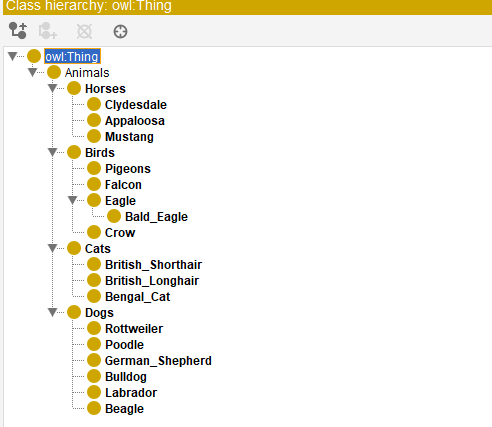
\includegraphics[scale=0.5]{Graphics/simple_ontology_owlviz.png}
\end{figure}

Die für diesen Zweck erstellte Ontologie, soll eine einfach Darstellung verschiedener Tierarten sein. 
Es gibt die Oberklassen Pferde, Vögel, Katzen und Hunde, sowie Unterklassen wie zum Beispiel die Klasse Labrador und Beagle, was Unterklassen von der Oberklasse Hund sind.
Diese Ontologie stellt keine komplizierten Relationen dar, beziehungsweise die einzelnen Klassen sind nur durch die Relation "subClassOf" miteinander verbunden.

\subsubsection*{Ontologie verarbeiten}
Im nächsten Schritt wird die Ontologie geparsed. Mit der Bibliothek rdfLib (VERWEIS), wird die Ontologie gelesen und queryable gemacht.
Nun möchte man alle Klassen dieser Ontologie erhalten, sowie die zugehörigen Relationen. Diese werden dann in einer Liste gespeichert, welche für die Visualisierung des Graphen im FrontEnd wichtig werden.

\begin{figure}[!ht]
    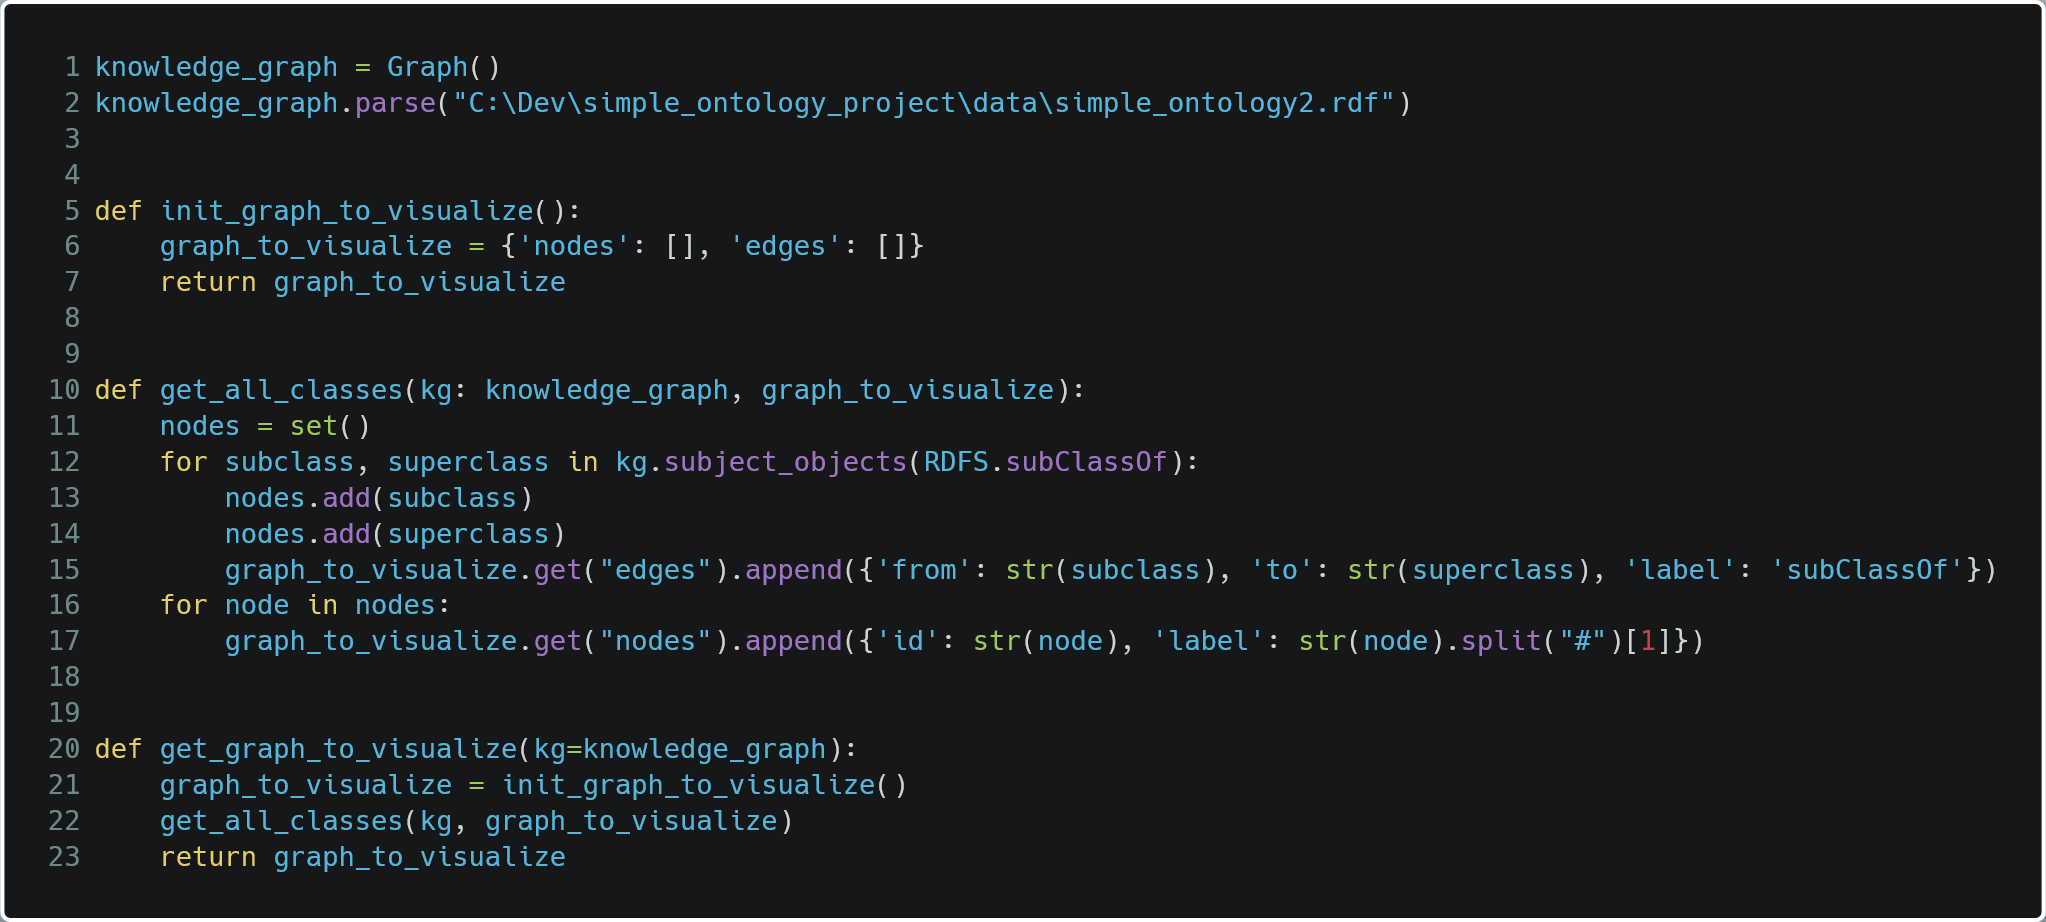
\includegraphics[scale=0.17]{Graphics/simple_ontology_graph_init.png}
    \end{figure}
    
\begin{itemize}
    \item Zeile 1 und 2: Es wird ein Graph erstellt, die Ontologie wird geparsed und zu diesem Graphen eingefügt
    \item Zeile 5 bis 7: Diese Funktion dient zur Weitergabe der Knoten und Kantenmenge für die Visualisierung des Graphen. Die Knoten repräsentieren die Klassen, die Kanten wiederrum die Relationen.
    \item Zeile 10 bis 17: Diese Funktion durchsucht den Graphen nach allen Klassen, diese Klassen unterscheiden sich zwischen Oberklasse und Unterklasse. Die Kanten zeigen dann von einer Oberklasse zur zugehörigen Unterklasse. Beide Klassen werden ebenfalls zu einer Liste der Knoten hinzugefügt.
    \item Zeile 20 bis 23: Die Menge der Knoten und Kanten werden für den Graphen initialisiert und stehen nun bereit für die Visualisierung.
\end{itemize}

Somit wurde die Verarbeitung der Ontologie für die Menge der Knoten und Kanten für die Visualisierung abgeschlossen. Nun möchte man diese Mengen visualieren.

\subsubsection*{From Backend to FrontEnd: Visualisierung}

Zur Erinnerung: Das Framework, welches wir nutzen ist Flask, damit kommunizieren wir zwischen dem FrontEnd, welches aus HTML, CSS und JavaScript besteht und unserem Backend, wo der Graph für die Visualisierung vorbereitet wird.
Zunächst erklären wir die Kommunikation mit dem FrontEnd
\begin{figure}[!ht]
    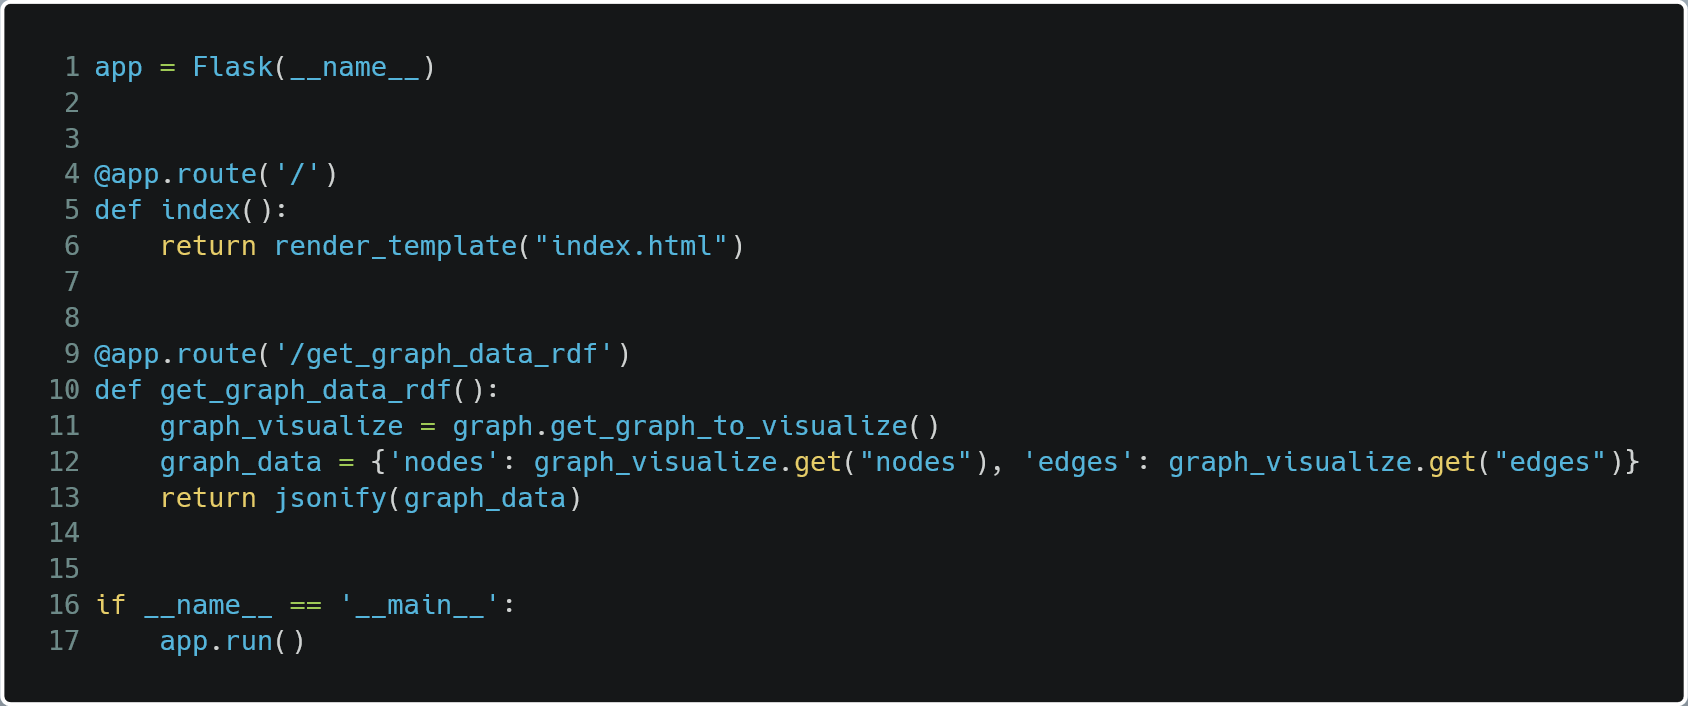
\includegraphics[scale=0.2]{Graphics/simple_ontology_flask.png}
    \end{figure}
    
\begin{itemize}
    \item Zeile 1 bis 6: Beim Starten der Anwendung, wird die HTML Seite "index.html" aufgerufen.
    \item Zeile 9 bis 17: Bei einem Aufruf der Funktion $"get\_graph\_data\_rdf"$, wird die Menge der Knoten und Kanten abgerufen, in einem Format, welches von der JavaScript Bibliothek vis.js verarbeitet werden kann.
\end{itemize}

Die Funktion "get\_graph\_data\_rdf" wird im FrontEnd JavaScript aufgerufen.
\begin{figure}[!ht]
    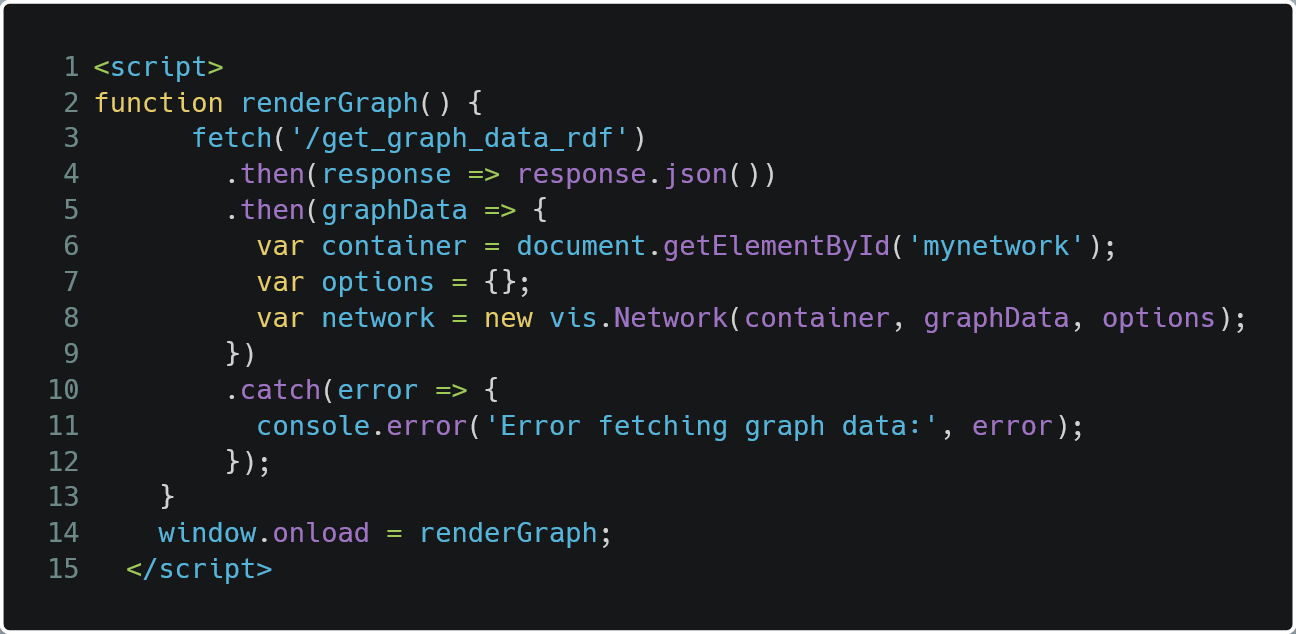
\includegraphics[scale=0.23]{Graphics/simple_ontology_js.png}
    \end{figure}

Der Graph wird erstellt mit den Daten, welche aus dem Output der Funktion $"get\_graph\_data\_rdf"$ entnommen wurden.
In Zeile 14 wird festgelegt, dass die Funktion zum rendern des Graphen, direkt beim Laden der HTML-Seite aufgerufen wird.

\begin{figure}[!ht]
    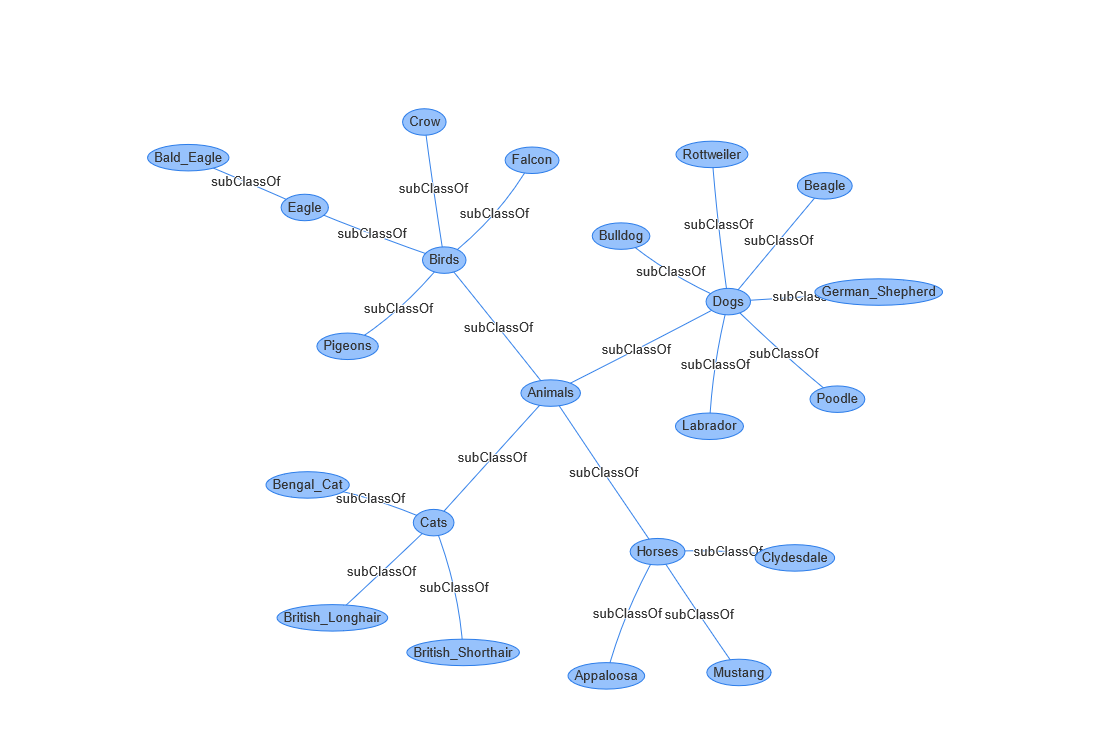
\includegraphics[scale=0.45]{Graphics/simple_graph.png}
    \end{figure}


 Dieses Beispiel zeigte den Weg zur Visualisierung einer einfachen Ontologie. 
 Allerdings sind die Ontologien, welche wir im Laufe der implementierung getestet haben viel komplizierter und brauchten verschiedene spezifische Implemetierungen um diese zu visualieren.
 Außerdem haben wir auch für die Visualisierung selbst einige Verbesserungen gegenüber dem Standartgraphen unternommen. 
 Die Implemetierung des Backends, sowie der 3 verschiedenen Funktionen (HINWEIS AUF MAIN FUNCTIIONS) wird im nächsten Abschnitt Detaillierterer beschrieben.
\subsection*{Implemetierung}
In diesem Abschnitt gehen wir auf ein triviales Beispiel der Implemetierung ein, um zu verdeutlichen, wie von der Verarbeitung der Wissensbasis, zum visualierten Graphen resultiert.
Detailliertere Einblicke gewähren wir in den einzelnen Abschnitten im nächsten Abschnitt "OWLVisualizer Framework".

Die Ontologie die zu dem gegebenen Zeitpunkt verarbeitet werden soll, befindet sich im data Ordner des Projekts. Somit beschränken wir uns nicht auf bestimmte Ontologien, sondern können beliebige Ontologien vearbeiten.
Diese Ontologie wird dann gelesen und geparsed mit Hilfe der Bibliothek rdfLib.

HIER BILD VOM CODE

Im nächsten Schritt wird es uns möglich die Ontologie zu queryien um so die Klassen und Relationen zu bestimmen. Je nach Aufbau der Ontologie, kann es vorkommen, dass zum Beispiel bei komplizierten Relationen Blank Nodes auftauchen, die nichts aussagend sind, sondern nur auf weitere Relationen hinweisen. Dieses Phänomen wird im Abschnitt "Visualisierung" näher betrachtet.
Im Graphen stellen die Klassen Knoten dar und die Relationen die Kanten. Somit benötigen wir 2 Mengen, eine Menge für die Knoten und eine Menge für die Kanten.

BILD HIER VOM CODE

Die Frontend Bibliothek vis.js benötigt diese 2 Mengen um einen Graphen zu erstellen. Außerdem können verschiedene Optionen mit angegeben werden um den Graphen zu verändern. Einige Optionen sind wichtig für die Performance des Graphen, dies wird im Abschnitt "Performance" näher erläutert.

BILD VON JS DATA FETCH.
\section*{The OWLVisualizer Framework}

\subsection*{Functionalities}

\subsection*{Visualisierung}

\subsection*{Query Builder}

\subsection*{Inference Query}

\subsection*{Performance}